\documentclass[10pt, a4paper, twosize]{article}
%\documentclass[12pt, a4paper, twoside]{book}

\usepackage{helvet}
\usepackage{hyperref}
\usepackage{graphicx}
\usepackage{listings}
\usepackage{textcomp}
\usepackage[
	a4paper,
	outer=2cm,
	inner=4cm,
	top=2cm,
	bottom=2cm
]{geometry}
\usepackage{float}
\usepackage{tabularx}
\usepackage[disable]{todonotes}
\usepackage{color, soul}
\usepackage{amsmath}
%\usepackage{algorithmicx}
%\usepackage[noend]{algpseudocode}
%\usepackage{algorithm}
\usepackage{framed}
\usepackage{subcaption}
\usepackage{titlepic}
\usepackage{fancyhdr}
\usepackage[simplified]{styles/pgf-umlcd}
\usepackage{shorttoc}
\usepackage{url}
\usepackage{paralist}
\usepackage[]{algorithm2e}
\definecolor{grey}{rgb}{0.9, 0.9, 0.9}
\definecolor{dkgreen}{rgb}{0,0.6,0}
\definecolor{dkred}{rgb}{0.6,0,0.0}

\lstdefinestyle{DOS}
{
    backgroundcolor=\color{black},
    basicstyle=\scriptsize\color{white}\ttfamily,
    stringstyle=\color{white},
    keywords={}
}

\lstdefinestyle{makefile}
{
    numberblanklines=false,
    language=make,
    tabsize=4,
    keywordstyle=\color{red},
    identifierstyle= %plain identifiers for make
}

\lstset{
  language=Java,                % the language of the code
  basicstyle=\footnotesize\ttfamily,
  numbers=left,                   % where to put the line-numbers
  stepnumber=1,                   % the step between two line-numbers. If it's 1, each line
  numbersep=5pt,                  % how far the line-numbers are from the code
  backgroundcolor=\color{white},      % choose the background color. You must add \usepackage{color}
  showspaces=false,               % show spaces adding particular underscores
  showstringspaces=false,         % underline spaces within strings
  showtabs=false,                 % show tabs within strings adding particular underscores
  frame=single,                   % adds a frame around the code
  rulecolor=\color{black},        % if not set, the frame-color may be changed on line-breaks within not-black text (e.g. comments (green here))
  tabsize=2,                      % sets default tabsize to 2 spaces
  captionpos=b,                   % sets the caption-position to bottom
  breaklines=true,                % sets automatic line breaking
  breakatwhitespace=false,        % sets if automatic breaks should only happen at whitespace
  keywordstyle=\color{blue},          % keyword style
  commentstyle=\color{dkgreen},       % comment style
  stringstyle=\color{dkred},         % string literal style
  columns=fixed,
  extendedchars=true,
  frame=single,
}

%\renewcommand{\chaptername}{Topic}

%% New definitions
%\algnewcommand\algorithmicswitch{\textbf{switch}}
%\algnewcommand\algorithmiccase{\textbf{case}}
%\algnewcommand\algorithmicassert{\texttt{assert}}
%\algnewcommand\Assert[1]{\State \algorithmicassert(#1)}%
%% New "environments"
%\algdef{SE}[SWITCH]{Switch}{EndSwitch}[1]{\algorithmicswitch\ #1\ \algorithmicdo}{\algorithmicend\ \algorithmicswitch}%
%\algdef{SE}[CASE]{Case}{EndCase}[1]{\algorithmiccase\ #1}{\algorithmicend\ \algorithmiccase}%
%\algtext*{EndSwitch}%
%\algtext*{EndCase}%

\pagestyle{fancy}
\fancyhf{}
\fancyhead[RO, LE]{\small \rightmark}
\fancyfoot[RO, LE]{\small \thepage}

\begin{document}

%\frontmatter

\begin{titlepage}
\vspace*{5cm}
\begin{center}
\includegraphics[width=.5\textwidth]{images/EdNapUniLogoCMYK}~\\[1cm]

\textsc{\Large Edinburgh Napier University}\\[1.5cm]

\textsc{\LARGE \bfseries SET08122 Algorithms \& Data Structures}\\[0.5cm]

\hrulefill \\[0.4cm]
{\huge \bfseries Lab 11 -- Expression processing \\[0.4cm] }
\hrulefill \\[1.5cm]

\begin{minipage}{0.4\textwidth}
\begin{flushleft} \large
\textbf{Dr Simon Powers} \\
\end{flushleft}
\end{minipage}

\vfill

\end{center}
\end{titlepage}

%\shorttoc{Overview}{0}

%\setcounter{tocdepth}{2}
%\cleardoublepage
%\tableofcontents
%\listoffigures
%\listofalgorithms
%\addtocontents{toc}{~\hfill\textbf{Page}\par}

%\mainmatter

%\input{sections/labs/04_ui}

\section{Aims}
\paragraph{} At the end of this topic you will be able to:

\begin{itemize}
\item Process expressions written in postfix notation using a stack.
\item Construct an expression tree using a stack.
\item Evaluate an expression tree.
\item Traverse an expression tree in pre-order, in-order, and post-order, to produce prefix, infix and postfix representations of the expression.
\end{itemize}

\section{Expression processing}
The aim of this unit is to examine and implement different algorithms for processing arithmetic operations on a computer. As a side-effect, we will gain plenty of practise with using stacks and trees, looking at some algorithms that make use of them (both at the same time!).

Expression processing is an important part of compiling or interpreting programs, as well as its obvious application in calculators of various shapes and sizes. Traditionally in mathematics we write expressions in infix notation, where an operator (e.g. + or *) is placed between the two operands (numbers) that it applies to. However, expressions written in infix notation are not well-suited to processing by a computer, because they require parentheses to determine the order of evaluation. For example, consider the expression:
74 - 10 / 32 
If we wish to specify that 10 should be subtracted from 74 and the result then divided by 32 then we need to use parentheses around (74 - 10). Having to deal with parentheses to determine the order of evaluation makes evaluating the expression unnecessarily difficult. There are two other forms of notation that get around this problem, where parentheses are never needed. 

The first of these is \emph{prefix} notation (also known as Polish notation, after the nationality of its inventor). In this notation, an operator precedes its operands. For example, the infix expression (74 - 10) / 32 would become / - 74 10 32. On the other hand, the infix expression 74 - (10 / 32) would be written as - 74 / 10 32. The second notation, which we will concentrate on in this lab, is known as \emph{postfix} (or Reverse Polish) notation. In postfix notation, operators follow their operands. The infix expression (74 - 10) / 32 would be written as 74 10 - 32 /, while the infix expression 74 - (10 / 32)  would be written as 74 10 32 / -.

Postfix expressions are easy to evaluate with an \emph{abstract stack machine}, a model of computation used by compiler and hand-held calculators. To process a postfix expression using an abstract stack machine, we proceed as follows. Move from left to right through the expression. Push values onto the stack until an operator is encountered. Next, the number of operands required by the operator (which will be two for a binary operator such as + or *) are popped from the stack, the operator is applied to them, and the result is pushed back onto the stack. This procedure is repeated until the entire expression has been processed, at which point the value of the evaluated expression is the sole item remaining on the stack.

\textbf{Exercise}: Write a program in C to read in an expression written in postfix notation from the console, and process it using the above algorithm. Check your implementation by evaluating the following postfix expression: 74 10 - 32 / 23 17 + *. The correct answer is 80.

\section{Expression trees}
Expressions are often represented in a computer using an \emph{expression tree}. Figure 1 shows an example expression tree. An expression tree is a binary tree consisting of two types of objects: \emph{operators} and \emph{terminal values}. Terminal values (operands) are the leaf nodes of the tree. The idea behind an expression tree is simple: the children of a node are the operands of the operator stored in that node. Operands may be terminal values, or they may be other expressions themselves.   
  \begin{figure}
        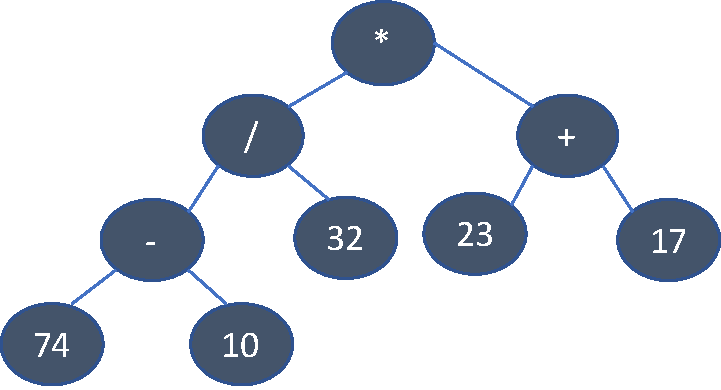
\includegraphics[scale=0.8]{expression_tree}
        \caption{Figure 1: An expression tree for the expression ((74 - 10) / 32) * (23 + 17).}
        \end{figure}

We can build an expression tree using Algorithm 1, which takes as input an expression in postfix notation, and returns the root node of the corresponding expression tree. The expression tree can then be evaluated according to Algorithm 2. In a compiler, the expression tree would be used to generate assembly code to evaluate the expression.

\begin{algorithm}[h]
\KwIn{expression string in postfix form}
\While{not at end of string}{
\eIf{token is an operand}{
create a new leaf node storing its value\;
set left and right child pointers to NULL\;
push the new node onto the stack\;
}
{
create a new node storing the operator\;
pop a node from the stack, attach to right child pointer\;
pop a node from the stack, attach to left child pointer\;
push the new node onto the stack\;

}
\Return{the single node remaining on the stack, 
which is the root of the expression tree}
}
\caption{An algorithm to build an expression tree.}
\end{algorithm}

\begin{algorithm}[h]
\KwIn{tree -- the root note of the tree}
\If{tree is not null}
{
\eIf{data field of tree is an operand}
{
\Return{data field of tree}
}
{
a = call the algorithm recursively on the left child of tree\;
b = call the algorithm recursively on the right child of tree\;
operator = data field of tree\;
\Return{a operator b}
}
}
\caption{An algorithm to evaluate an expression tree.}
\end{algorithm}


\subsection{Traversing expression trees}
Expression trees allow us to very easily produce prefix, infix, and postfix representations of the expression. To produce a prefix representation, traverse the tree in \emph{preorder} following Algorithm 3. To produce a postfix representation, traverse the tree in \emph{postorder} according to Algorithm 4. 
\begin{algorithm}[h]
\KwIn{tree -- the root node of the tree}
\If{tree is not empty}{
print (tree token)\;
call recursively on the left child of tree\;
call recursively on the right child of tree\;
}
\caption{Print a tree in preorder to produce a prefix expression.}	
\end{algorithm}

\begin{algorithm}[h]
\KwIn{tree -- the root node of the tree}
\If{tree is not empty}{
call recursively on the left child of tree\;
call recursively on the right child of tree\;
print (tree token)\;
}
\caption{Print a tree in postorder to produce a postfix expression.}	
\end{algorithm}

Producing an infix representation is more complex, because parentheses are necessary to disambiguate the order of evaluation. Parentheses need to be placed around each subtree. Algorithm 5 performs an \emph{inorder} traversal of the tree that adds parentheses at the appropriate places. 

\begin{algorithm}[h]
\KwIn{tree -- the root node of the tree}
\If{tree is not empty}{
\If{tree token is an operator}{
print(open parenthesis)
}
call recursively on the left child of tree\;
print (tree token)\;
call recursively on the right child of tree\;
\If{tree token is an operator}{
print(close parenthesis)
}
}
\caption{Print a tree in inorder to produce an infix expression.}	
\end{algorithm}


\textbf{Exercise:} Implement the algorithm to build an expression tree in C. You can use the binary\_tree\_node struct that you developed in Lab 05 to represent the nodes of the tree. You can ue the data field to store operators or operands (remember that a character is just a small \texttt{int} in memory, so you can store characters such as `+' in an \texttt{int} in C). You should test your implementation by using Algorithm 1 to produce the expression tree for our favourite expression, 74 10 - 32 / 23 17 + *. Check that Algorithm 2 evaluates the expression tree correctly, and that the expressions produced by Algorithms 3, 4 and 5 are correct.

\bibliographystyle{plain}

\bibliography{workbook}

\end{document}


%\begin{framed}
%HELLO
%\end{framed}


